\item In Problem 21, how many different paths are there from A to B that go through the point circled in the following lattice?
\[
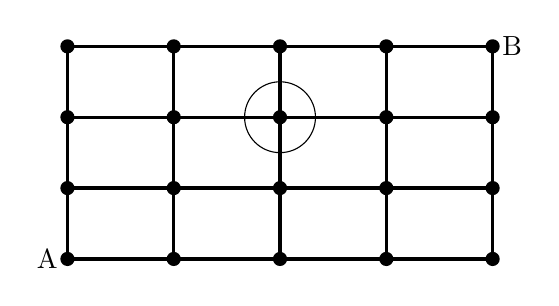
\begin{tikzpicture}[scale=0.9]
    \draw[very thick, xstep=1.5] (0, 0) grid (6, 3);
    \foreach \i in {0, 1.5, ..., 6} {
        \foreach \j in {0, 1, 2, 3} {
            \fill (\i, \j) circle (0.1);
        }
    }
    \node[anchor=east] at (0, 0) {A};
    \node[anchor=west] at (6, 3) {B};
    \draw (3, 2) circle (0.5);
\end{tikzpicture}
\]

Considerar la secuencia
\[ \rightarrow\ \rightarrow\ \uparrow\ \uparrow \]
las permutaciones únicas de esta secuencia son los posibles caminos de $A$ al punto marcado.

Considerar la secuencia
\[ \rightarrow\ \rightarrow\ \uparrow \]
las permutaciones únicas de esta secuencia son los posibles caminos del punto marcado a B.

Luego sigue que hay
\[ \frac{4!}{2! * 2!} * \frac{3!}{2!} \]
posibles caminos de A a B pasando por el punto marcado.